\documentclass[12pt]{article}

\usepackage{amsmath}
\usepackage{amssymb}
\usepackage{bm}
\usepackage{enumerate}
\usepackage{fancyvrb}
\usepackage[top=1in, bottom=1in, left=1in, right=1in]{geometry}
\usepackage{hyperref}
\usepackage{placeins}
\usepackage{tikz}
\usepackage{tikzsymbols}
\usepackage{todonotes}
\usepackage{bbm}
\usepackage{color}
\newcommand{\rmn}[1]{{\textcolor{blue}{\bf [{\sc rmn:} #1]}}}
\DeclareMathOperator*{\argmax}{arg\,max}

\usetikzlibrary{positioning,calc}
%%%%%%%%%
\usepackage[most]{tcolorbox}
\newtcolorbox[]{solution}[1][]{%
    breakable,
    enhanced,
    colback=white,
    title=Solution,
    #1
}
%%%%%%%%%%
\title{10-703 Deep Reinforcement Learning and Control\\
  Assignment 2: Model-Free Learning\\
  Spring 2018\\
}

\author{Bhargavi Paranjape, Aditya Siddhant}

\date{Febuary 21, 2018\\
  \hspace{1cm}\\
Due March 7, 2018}

\begin{document}

\maketitle

\section*{Instructions}

You have around 15 days from the release of the assignment until it is due. Refer to Grade-scope for the exact time due.  You may work in teams of \textbf{2} on this assignment. Only one person should submit the writeup and code on Gradescope. Additionally you should upload your code to Autolab, please make sure the same person who submitted the writeup and code to Gradescope is the one who submits it to Autolab.  Make sure you mark your partner as a collaborator on Gradescope (You do not need to do this in Autolab) and that both names are listed in the writeup.  Writeups should be typeset in Latex and submitted as PDF. All code, including auxiliary scripts used for testing should be
submitted with a README.

\section*{Introduction}

% what is the goal of this section.
In Homework 1, you learned about and implemented various model-based techniques to solve MDPs. These ``planning'' techniques work well when we have access to a model of the environment; however getting access to such a model is often unfeasible. In this Homework, you will explore an alternative to the model-based regime, i.e. model-free learning. 
In particular, you will learn about Temporal Difference learning and its variants, and implement a version of TD learning called Q-learning. We will look at implementing Q learning with both tabular methods and deep function approximators. 

You will work with the OpenAI Gym environments, and learn how to train a Q-network from state inputs on a gym environment. The goal is to understand and implement some of the techniques that were found to be important in practice to stabilize training and achieve better performance. We also expect you to get comfortable using Tensorflow or Keras to experiment with different architectures, and understand how to analyze your network's final performance and learning behavior. 

Please write your code in the file \texttt{DQN\_Implementation.py}, the template code provided inside is just there to give you an idea on how you can structure your code but is not mandatory to use.

\section*{Background in Q-learning and Variants}

Function approximators have proved to be very useful in the reinforcement learning setting. Typically, one represents Q-functions using a class of parametrized function approximators $\mathcal Q = \{ Q _w \mid w \in \mathbb R ^p \}$, where $p$ is the number of parameters. Remember that in the \emph{tabular setting}, given a $4$-tuple of sampled experience $(s, a, r, s')$, the vanilla Q-learning update is 
%% is for a pair (s, a, r, s')
\begin{align}
	Q(s, a) := Q(s, a) + 
		\alpha \left( 
			r + \gamma \max _{a' \in A} Q(s', a') 
				- Q(s, a) 
		\right)   ,
	\label{eq:tab_qlearn}
\end{align}
where $\alpha \in \mathbb R$ is the learning rate. In the \emph{function approximation setting}, the update is similar: 
\begin{align}
	w := w + 
		\alpha \left( 
			r + \gamma \max _{a' \in A} Q _w(s', a') 
				- Q _w(s, a) 
		\right) \nabla _w 
			Q _w (s, a) .
	\label{eq:fapp_qlearn}
\end{align}
% this part is kind of unnecessary.
Q-learning can be seem as a 
pseudo stochastic gradient descent step on 
\begin{align*}
	\ell (w) = \mathbb E _{s, a, r, s'} 
		\left( 
			r + \gamma \max _{a' \in A} Q _w(s', a')
				- Q _w(s, a) 
		\right) ^2 ,
\end{align*}
where the dependency of $\max _{a' \in A} Q _w(s', a')$ on $w$ is ignored, i.e., it is treated as a fixed target. Many of the methods that you will implement in this homework are variants of update \eqref{eq:fapp_qlearn}. We recommend reading through the \emph{deep Q-learning implementation} described in~\cite{mnih2013playing, mnih2015human}. 

% BEGIN comment out Double DQN
\iffalse 
% namely in the way the targets are constructed and maintained.
maintains two Q-networks: the online network, which plays the same role of the $Q _w$ terms  $Q _w(s, a)$ and $\nabla _w Q _w (s, a)$ in update~\eqref{eq:fapp_qlearn}, and the target network, which is used in the target in update~\eqref{eq:fapp_qlearn}. The update in this case is 
\begin{align}
	w := w + 
		\alpha \left( 
			r + \gamma \max _{a' \in A} Q _{w ^-} (s', a') 
				- Q _w(s, a) 
		\right) \nabla _w 
			Q _w (s, a) .
\end{align}
The target Q-network is assigned every so often to be equal to the online Q-network, and is kept frozen until the next assignment. This helps the stability of the learning procedure, as with deep learning function approximators, updating the target Q-network with every update to the online Q-network proves too unstable. 

\emph{Double Q-learning}~\cite{van2016deep} also maintains two Q-networks, but they do not play a fixed role as online and target networks as in~\cite{mnih2013playing, mnih2015human}. Let us call the networks $Q _{w _1}$ and $Q _{w _2}$; at each update step, we flip a fair coin and either do 
\begin{align}
	{w _1} := {w _1} + 
		\alpha \left( 
			r + \gamma Q _{w _2}
				(
					s', \argmax _{a' \in A} Q _{w _1} (s', a')
				) 
				- Q _{w _1}(s, a) 
		\right) \nabla _{w _1} 
			Q _{w _1} (s, a) 
\end{align}
or 
\begin{align*}
	{w _2} := {w _2} + 
		\alpha \left( 
			r + \gamma Q _{w _1}
				(
					s', \argmax _{a' \in A} Q _{w _2} (s', a')
				) 
				- Q _{w _2}(s, a) 
		\right) \nabla _{w _2} 
			Q _{w _2} (s, a) .	
\end{align*}
As at each update the role of $Q _{w _1}$ and $Q _{w _2}$ is determined stochastically with probability $0.5$, these networks play a symmetric role. This helps with the over-optimism of the targets in update~\eqref{eq:fapp_qlearn}.
\fi
% END of comment out Double DQN

In this homework, we will also ask you to implement the \emph{dueling deep Q-network} described in~\cite{wang2015dueling}. This amounts to a slightly different Q-network architecture from the 
one in~\cite{mnih2013playing, mnih2015human}. Most models will be trained using \emph{experience replay}~\cite{mnih2013playing, mnih2015human}, meaning that the $4$-tuples $(s, a, r, s')$ will be sampled from the replay buffer rather than coming directly from the online experience of the agent.

\pagebreak[4]

\section{Theory Questions}
\subsection*{Question 1.a \textbf{[5pts]}}

Consider a sequence of streaming data points $\mathbf{X}: \{ x_1, x_2, x_3, ... x_N\}$. At any given time instant $k$, one has access to data points $\{ x_1, x_2, ... x_k\}$; but not $\{ x_{k+1}, ... x_N\}$. 
Prove that the mean $\mu_k$ of the available data may be computed incrementally (online) at every time step $k$, in the form: $\mu_k =\mu_{k-1} + f(\mu_{k-1}, x_k)$.\\

\noindent
\begin{solution}
From the definition of average, we have:
$$\mu_{k-1} = \frac{x_1 + x_2 + ... + x_{k-1} }{k-1}$$
$$(k-1)\mu_{k-1} = x_1 + x_2 + ... + x_{k-1}$$
Similarly, 
$$\mu_{k} = \frac{x_1 + x_2 + ... + x_{k-1} + x_k}{k}$$
$$k\mu_{k} = x_1 + x_2 + ... + x_{k-1} + x_k$$
$$k\mu_{k} = (k-1)\mu_{k-1} + x_k$$
$$\mu_{k} = \frac{(k-1)\mu_{k-1} + x_k}{k}$$
$$\mu_{k} = \mu_{k-1} + \frac{x_k - \mu_{k-1}}{k}$$
$$\mu_{k} = \mu_{k-1} + f(\mu_{k-1}, x_k)$$
where
$$f(\mu_{k-1}, x_k) = \frac{x_k - \mu_{k-1}}{k}$$
Hence mean $\mu_k$ can be computed  incrementally (online) at every time step $k$ using the above update equation with $f$ as defined.
\end{solution}

\pagebreak[4]

\subsection*{Question 1.b \textbf{[5pts]}}
The function $f(x_k, \mu_{k-1})$ represents the error between the current estimate of the mean, $\mu_{k-1}$, and the true mean at time $k$, $\mu_k$. Consider the following scenario - an agent follows some policy in its environment, and receives a return $G_t$ from an episode starting at state $s_t$. We would like to update the value of state $s_t$, $V(s_t)$, using the newly obtained $G_t$. 

\begin{itemize}
    \item Treating the update of $V(s_t)$ as an online learning problem, where $G_t$ is the newly received data point, show that the current estimate of the value of the state $V(s_t)$ can be updated in a form analogous to Question 1.a. You may assume that the state $s_t$ has been visited $N(s_t)$ number of times.
    
    \item What is the error function $f$? What does the update you derived resemble?  
\end{itemize}

\noindent
\begin{solution}
Let $s_t = s$ and $N(s_t) = k$ at time $t$. Hence, state $s$ was encountered $k$ number of times before time $t$ with returns from episodes for these $k$ occurrences being ${G_1, G_2, ... , G_k}$. Hence at time $t$, we have,
$$V(s_t) = \frac{G_1 + G_2 + ... + G_k}{k}$$
At time $t$, the datapoint $G_t$ is added to this average to compute a new value function for state $s_t = s$. Let's call it $V_{new}(s_t)$. Then,
$$V_{new}(s_t) = \frac{G_1 + G_2 + ... + G_k + G_t}{k+1}$$
Again we have,
$$(k+1)V_{new}(s_t) = kV(s_t) + G_t$$
$$(k+1)V_{new}(s_t) = (k + 1 - 1)V(s_t) + G_t$$
$$(k+1)V_{new}(s_t) = (k + 1)V(s_t) + G_t - V(s_t)$$
$$V_{new}(s_t) = \frac{(k + 1)V(s_t) + G_t - V(s_t)}{(k+1)}$$
$$V_{new}(s_t) = V(s_t) + \frac{G_t - V(s_t)}{(k+1)}$$
$$N_{new}(s_t) = k+1$$
Hence we have,
$$V_{new}(s_t) = V(s_t) + \frac{G_t - V(s_t)}{N_{new}(s_t)}$$
This update equation for $V(s_t)$ is similar to the Monte-Carlo update equation of the form:
$$V_{new}(s_t) = V(s_t) + \frac{1}{\alpha}(G_t - V(s_t))$$
with $\frac{1}{N(s_t)} = \alpha$
\end{solution}

\pagebreak[4]

\subsection*{Question 1.c \textbf{[5pts]}}
The update you derived in Question 1.b is based on the return from the entire episode, $G_t$. However, this method only learns from the end of the episode. Instead, it is possible to accelerate the learning process by bootstrapping. 

\begin{enumerate}
    \item Consider the agent is in state $s_t$, takes an action $a_t$, and transitions to state $s_{t+1}$, receiving reward $r$. Write out the estimate of the return of this episode based on this reward $r$ and the current estimate of the value function $V$. 
    \item In the update from Question 1.b, replace the return $G_t$ with the above estimate of return, and write out the new update for the value function $V(s_t)$. What does this update resemble?
\end{enumerate}

\noindent
\begin{solution}
$G_t$ is the reward for the current episode starting at state $s_t$ at time $t$ and $V(s_{t+1})$ is the average expected reward for this episode starting at state $s_{t+1}$ at time $t+1$ after a reward $r$ has already been achieved. Hence, $G_t$ will include the reward $r$ and the expected reward from next time step $V(s_{t+1})$. I.e.,
% $$G_t = \mathbb{E}_{a \in A}r(s_t, a) + V(s_{t+1})$$
$$G_t = r + V(s_{t+1})$$
Putting this value for $G_t$ in previous update equation, we get:
$$V_{new}(s_t) = V(s_t) + \frac{r + V(s_{t+1}) - V(s_t)}{N_{new}(s_t)}$$
This update equation for $V(s_t)$ is similar to the Temporal Difference[TD(0)] update equation of the form:
$$V_{new}(s_t) = V(s_t) + \frac{1}{\alpha}(r + V(s_{t+1}) - V(s_t))$$
with $\frac{1}{N(s_t)} = \alpha$
\end{solution}

\pagebreak[4]

\subsection*{Question 2.a \textbf{[5pts]}}
Update~\ref{eq:tab_qlearn} defines the TD update when the representation of the states and actions are in tabular form. Show that for a certain construction of the feature function $\phi$, the tabular representation representation is a special case of the TD update~\ref{eq:fapp_qlearn} where the function in $\mathcal Q$ is of the form $Q _w(s, a) = w ^T \phi(s, a)$. Give detailed description about your feature function and your proof for equivalence to earn full credits. \\

\noindent
\begin{solution}
Update 1 is of the form:
	$$Q'(s, a) := Q(s, a) + 
		\alpha \left( 
			r + \gamma \max _{a' \in A} Q(s', a') 
				- Q(s, a) 
		\right)$$
We have,
$$Q_{w}(s, a) = w^T \phi(s, a)$$
$$\nabla _w Q_w (s, a)  = \phi(s, a)^T $$
Using the update equation for w and the linear function for 
	$$w' := w + 
		\alpha \left( 
			r + \gamma \max _{a' \in A} Q _w(s', a') 
				- Q _w(s, a) 
		\right) \nabla _w 
			Q _w (s, a)$$
	$$w' := w + 
		\alpha \left( 
			r + \gamma \max _{a' \in A} Q _w(s', a') 
				- Q _w(s, a) 
		\right)\phi(s, a)^T $$
Substituting the updated value $w'$ to compute $Q'_{w}(s, a)$, we get
$$Q'_{w}(s, a) = w'^T\phi(s, a)$$
	$$Q'_{w}(s, a) := \left[w + 
		\alpha \left( 
			r + \gamma \max _{a' \in A} Q _w(s', a') 
				- Q _w(s, a) 
		\right)\phi(s, a)\right]^T\phi(s, a)$$

	$$Q'_{w}(s, a) := w^T\phi(s, a) + 
		\alpha \left( 
			r + \gamma \max _{a' \in A} Q _w(s', a') 
				- Q _w(s, a) 
		\right)\phi(s, a)^T\phi(s, a)$$
	$$Q'_{w}(s, a) := Q_{w}(s, a) + 
		\alpha \left( 
			r + \gamma \max _{a' \in A} Q _w(s', a') 
				- Q _w(s, a) 
		\right)\phi(s, a)^T\phi(s, a)$$
In order equate this value for $Q'_{w}(s, a)$ to Update 1, we get:
$$\phi(s, a)^T\phi(s, a) = 1$$
That is:
$$||\phi(s, a)|| = 1$$
Hence, if the feature vectors are normalized to norm-1, the function approximation setting reduces to the tabular setting
\end{solution}

\pagebreak[4]

\subsection*{Question 2.b \textbf{[5pts]}}
State aggregation improves generalization by grouping states together, with one table entry used for each group. Let $\mathcal{X}: s \to x$ be the grouping function that maps a input state $s$ to its group $x$ and usually, the number of groups $|X| \ll |S|$. During training, whenever a state in a group is encountered, the groups' entry and the action $a$ is used to determine the state's value, and when the state is updated, the group's entry is updated. Assume $\mathcal Q$ is still in the the form $Q _w(s, a) = w ^T \phi(s, a)$. Show that a tabular representation with state aggregations is also a special case of TD update~\ref{eq:fapp_qlearn} under certain construction of feature function $\phi$. Give detailed description about your feature function and your proof for equivalence to earn full credits.

\noindent

\begin{solution}
Consider the set of states $S_x = {s_1, s_2, ..., s_k}$, that are all mapped to the group $x$. Then, 
$$\mathcal{X}(s) = x, \quad \forall s \in S_x$$
$$Q(s,a) = Q(x,a), \quad \forall s \in S_x$$
The weight update equation for every state $s$ in $S_x$ is then of the form:
	$$w' := w + 
		\alpha \left( 
			r + \gamma \max _{a' \in A} Q _w(\mathcal{X}(s'), a') 
				- Q_w(x, a) 
		\right)\phi(s, a)^T \quad \forall s \in S_x $$
And the updated value for $Q'_{w}(s, a)$ [$Q'_{w}(x, a)$] is as follows:
	$$Q'_{w}(s, a) := w^T\phi(s, a) + 
		\alpha \left( 
			r + \gamma \max _{a' \in A} Q _w(\mathcal{X}(s'), a') 
				- Q _w(x, a) 
		\right)\phi(s, a)^T\phi(s, a) \quad \forall s \in S_x $$
	$$Q'_{w}(s, a) := Q_w(x,a) + 
		\alpha \left( 
			r + \gamma \max _{a' \in A} Q _w(\mathcal{X}(s'), a') 
				- Q _w(x, a) 
		\right)\phi(s, a)^T\phi(s, a) \quad \forall s \in S_x$$
In order equate this value for $Q'_{w}(s, a)$ to Update 1, the following conditions must hold:
$$Q_w(x,a) = Q_w(s,a) = w^T\phi(s, a) \quad \forall s \in S_x$$
and, 
$$||\phi(s, a)|| = 1$$ 
The first constraint implies that for all states that are mapped to the same group and hence have the same q-value, the feature function $\phi$ has to be identical for all these states. That is:
$$\phi(s, a) = \phi(s', a) = \phi(x,a) \quad \forall (s,s') \in S_x , a\in A$$
We can hence define feature functions over groups according to the mapping $\mathcal{X}$
Thus, if the feature vectors are normalized to norm-1 and all feature functions of states mapped to the same group are identical, the function approximation setting reduces to the tabular setting.
\end{solution}

\section{Programming Implementation}
For each of the experiments, we provide a detailed setting with values of different hyperparameters used and the reason for the choice of some of the hyperparameters. We also provide a plot of model performance which is measured by calculating expected rewards at regular intervals during training. Further, we analyze each of the models based on its loss, reward and the policy learned as suggested by the video recorded at different training stages.

\paragraph{Loss Function} We use Mean Squared Error (MSE) as the loss function for our experiments as minimizing MSE Loss is equivalent to the vanilla Q-learning update. The Vanilla Q-learning update is:
\begin{align*}
	Q_w^{t+1}(s, a) := Q_w^{t}(s, a) + 
		\alpha \left( 
			r + \gamma \max _{a' \in A} Q_w^t(s', a') 
				- Q_w^t(s, a) 
		\right)
\end{align*}
At convergence, $Q_w^{t+1}(s, a)$ should be equal to $Q_w^{t}(s, a)$ which implies that the second term on the RHS should be close to zero which is exactly what minimizing MSE Loss achieves.

\pagebreak[4]

\subsection{Linear Q-Network without Experience Replay}
\subsection*{CartPole-v0}
\paragraph{Experiment Setting} There were only four weights in the network one corresponding to each variable in the state and a bias. To learn these weights, we used Adam Optimizer with initial learning rate 0.0001 to optimize the loss. During training, we use an epsilon greedy policy and decay the value of $\epsilon$ from 0.5 to 0.05 linearly over 1 million weight updates. Discount factor was set to 0.99 and the model was trained for 500 episodes. Figure \ref{fig:01} shows the performance of the model after different number of weight updates to model.
\begin{figure}[h]
  \centering
  \vspace{-5mm}
  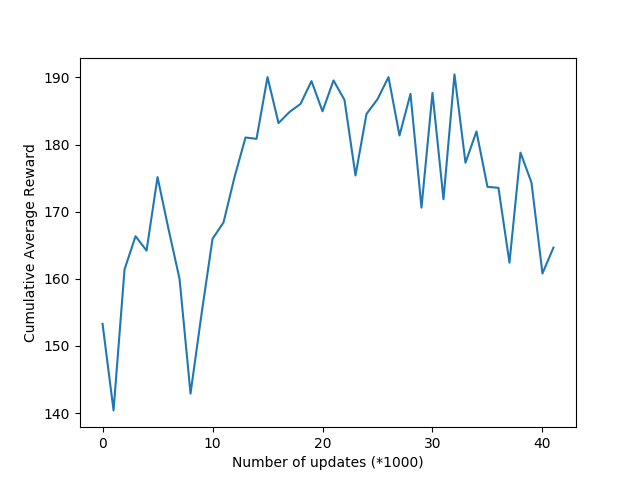
\includegraphics[width=0.8\linewidth]{figures/reward_plot_01.png}
  \caption{Performance of Linear Q-Network on CartPole}
  \label{fig:01}
\end{figure}
\paragraph{Observations} We found that the linear network is not able to solve CartPole environment with confidence. It is heavily dependent on initialization and with a bad initialization gets easily stuck in a local optima. Even when initialization is good, it is unable to give a consistent average reward of 200 and the performance oscillates a lot. Additionally, the model also unlearns the policy and the reward goes below 100 after training for some more time. We hypothesize that this might be due to inability of Optimizer (Gradient Descent) to exactly find the 4 parameters that can solve the environment because although the environment is linearly solvable, it is solvable only for few specific combinations of parameters in linear case which optimizer might not have been able to find. The rendering of the model learned shows that even when reward is high, the pole is very unstable and the cart keeps moving to one direction.\\
The set of linear equations for Q function which were found to solve the Cartpole-v0 environment are \cite{linearcart}:
$$ Q(s,0) = -s_3 - 3 \times s_2 $$
$$ Q(s,1) = s_3 + 3 \times s_2 $$
where 0,1 are left and right actions and the $s_2$ and $s_3$ denote pole position and pole velocity respectively.




\pagebreak[4]
\subsection*{MountainCar-v0}
\paragraph{Experimental Settings} There are two weights in the linear network excluding the bias term. We use the Adam optimizer over Smoother L1 Loss (Hubert Loss) with initial learning rate of 0.0001. During training, we use an epsilon greedy policy and decay the value of $\epsilon$ from 0.9 to 0.05 linearly over 1 million weight updates. To stabilize training we use a target network whose parameters are synced every 10,000 updates to the parameters of the learned q-function. We set discount factor to 1. We also employ the following reward function update rule at terminal states to further stabilize the training procedure:  Target is set to $r$ only if next state[0] $>$ 0.5 and is $r+γQ$ otherwise. We train for 10,000 episodes (2 million updates). Figure \ref{fig:mn02} shows the performance of the model measured in terms of average reward for 20 episodes after different number of weight updates to the model during training.\\
\begin{comment}
% This is supposed to be put in the table in Section 3 and we need to comment on that table too which I think we can do together or I can take care of that part. 
\textcolor{red}{Best Performance on validate:  Mean= -125.700000, Std= 17.286122}\\
\textcolor{red}{Best Performance on test: Mean= -124.710000, Std= 17.482731}\\
\textcolor{red}{Best Occurs after 40,000 updates ~200 episodes}
\end{comment}

\begin{figure}[h]
  \centering
  \vspace{-5mm}
  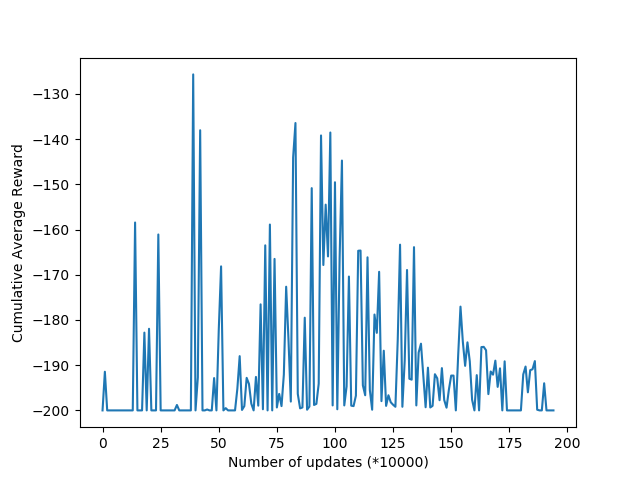
\includegraphics[width=0.8\linewidth]{figures/linear_noexp_hubert_target_reward_plot.png}
  \caption{Performance of Linear Q-Network on MountainCar with no experience replay}
  \label{fig:mn02}
\end{figure}

\paragraph{Observations} TBD

\pagebreak[4]

\subsection{Linear Q-Network with Experience Replay}
\subsection*{CartPole-v0}

\paragraph{Experiment Setting} Similar to the setting without experience replay, we used Adam Optimizer with initial learning rate 0.0001. Again, we use an epsilon greedy policy and decay the value of $\epsilon$ from 0.5 to 0.05 linearly over 1 million weight updates. We use a batch size of 32 for experience sampling, set the discount factor to 0.99 and train the model for 500 episodes. Figure \ref{fig:02} shows the performance of the model after different number of weight updates to model during training.
\begin{figure}[h]
  \centering
  \vspace{-5mm}
  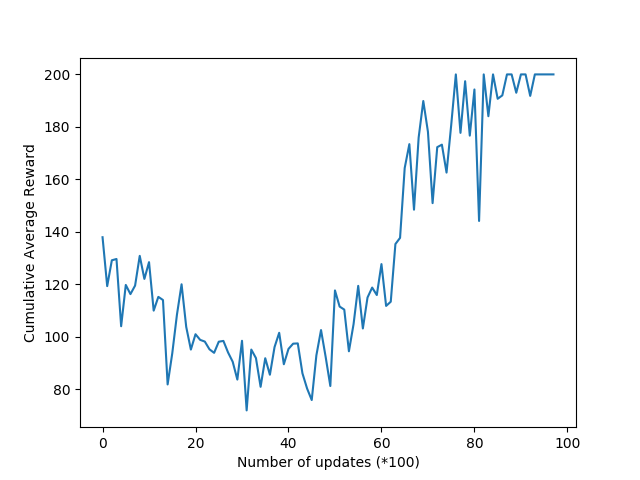
\includegraphics[width=0.8\linewidth]{figures/reward_plot_02.png}
  \caption{Performance of Linear Q-Network on CartPole with Experience Sampling}
  \label{fig:02}
\end{figure}
\paragraph{Observations} Experience replay does help the model and the model performs better than that without replay in a sense that the learned policy is sometimes able to reach a reward of 200. The number of episodes required for training is also reduced because of replay. However the model is still dependent on initialization and is able to reach only upto 100 reward for bad initializations which is again due to inefficiency of gradient descent. This model also unlearns the policy and the reward diminishes after training for some more time. To avoid this from happening, we use an early stopping criteria where we stop training if we get a average reward of more than 195 for 5 continuous evaluations. The rendering of the learned policy shows that the cart moves back and forth rapidly and pole is still oscillating a lot hinting that although reward is 200, the policy learned is still not what it ideally should be.

\pagebreak[4]
\subsection*{MountainCar-v0}

\paragraph{Experimental Settings} Similar to the setting without experience replay, we use Adam Optimizer (initial learning rate = 0.0001) with Hubert loss. We use an epsilon greedy policy for evaluation during training and decay the value of $\epsilon$ from 0.5 to 0.05 linearly over 1 million weight updates. We use batch size of 32

\pagebreak[4]
\subsection{Deep Q-Network}
\subsection*{CartPole-v0}
\paragraph{Setting} Since, we find out that linear network in not enough to convincingly solve the CartPole environment due to the non-linearity in the physics of the environment, we try a Multi-layer perceptron with 2 hidden layers to solve the problem. We have 16 units in both layers and we use ReLU as activation function for non-linearity. We use adam optimizer with initial learning rate 0.001. Again, we use an epsilon greedy policy and decay the value of $\epsilon$ from 0.5 to 0.05 linearly over 1 million weight updates. We use a batch size of 32 for experience replay and set discount factor to 0.99. Figure \ref{fig:03} shows the performance of the model after different number of weight updates to model during training.
\begin{figure}[h]
  \centering
  \vspace{-5mm}
  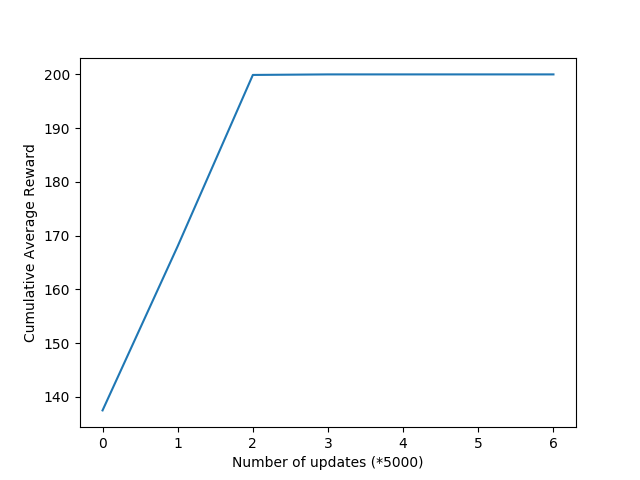
\includegraphics[width=0.8\linewidth]{figures/reward_plot_04.png}
  \caption{Performance of Deep Q-Network on CartPole with Experience Sampling}
  \label{fig:03}
\end{figure}
\paragraph{Observations} We find that Multi-layer Perceptron is able to fully solve the CartPole environment and able to obtain an average reward of 200 consistently irrespective of initialization. The average reward obtained is also stable for a long time and does not unlearn quickly as the linear ones do. Learning however takes more time as the number of parameters are more and as a reason, a higher learning rate (0.001) was used. Again, we use a stopping criteria to prevent the model from overfitting because the risk of overfitting is high due to higher number of parameters as compared to linear model. We stop training when we get a reward of 195 or more for 5 continuous evaluations. Finally, by examining the recording of the learned policy, we find that it is better than linear in the sense that pole does not oscillate and almost maintains its position. However, a caveat in the policy learned is that the cart tends to move in one direction either left or right in order to balance the pole.

\paragraph{Without Experience Replay} Additionally, we learn an MLP Q Network without experience replay and find that MLP is able to solve the environment without experience replay and in fact does better in terms of reward stability as compared to linear with experience replay and does not unlearn as fast as linear does. As compared to MLP with experience replay, it take more episodes to converge, The rewards are less stable and its policy is slightly inferior in sense that the pole oscillates a bit. Figure \ref{fig:04} shows the performance of the model after different number of weight updates to model during training.

\begin{figure}[h]
  \centering
  \vspace{-5mm}
  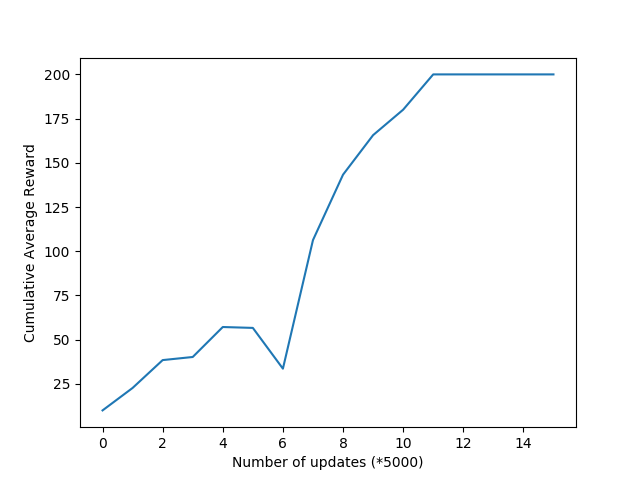
\includegraphics[width=0.8\linewidth]{figures/reward_plot_03.png}
  \caption{Performance of Deep Q-Network on CartPole without Experience Sampling}
  \label{fig:04}
\end{figure}

\pagebreak[4]
\subsection*{MountainCar-v0}

\pagebreak[4]
\subsection{Duelling Deep Q-Network}
\subsection*{CartPole-v0}
\paragraph{Setting} For the duelling dqn, we use a two layer MLP woith 16 units each as the shared architecture and then use tow MLPs of 1 layer with 16 units to compute advantage and value function. Similar to MLP, we use Adam Optimizer with initial learning rate of 0.001 and again, we use an epsilon greedy policy and decay the value of $\epsilon$ from 0.5 to 0.05 linearly over 1 million weight updates. Discount factor was set to 0.99 and We use a batch size of 32 for experience replay. Figure \ref{fig:05} shows the performance of the model after different number of weight updates to model during training.
\begin{figure}[h]
  \centering
  \vspace{-5mm}
  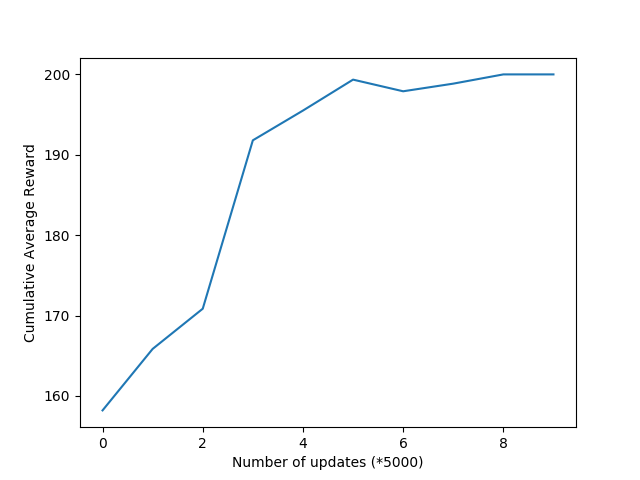
\includegraphics[width=0.8\linewidth]{figures/reward_plot_05.png}
  \caption{Performance of Duelling DQN on CartPole with Experience Sampling}
  \label{fig:05}
\end{figure}
\paragraph{Observations} We find that duelling dqn takes lesser number of episodes to learn and is as good as dqn in terms of reward stability. One interesting thing to note was that number of updates was higher than dqn even though episodes were less. Examining the plot, we find out that duelling dqn starts to learn very quickly and the reward go up to 193 just after first 5000 weight updates. Another interesting observation was the recording of the policy learned by duelling dqn. It was most stable of all the policies learned so far. The car position was also stable and so was the pole's angle. There were very small movements and the actions perfectly balanced the pole. 

\pagebreak[4]
\subsection*{MountainCar-v0}

\pagebreak[4]
\subsection{Deep Convolutional Double Q-Network}
\subsection*{SpaceInvaders-v0}

\pagebreak[4]
\section{Test Results}

\begin{table}[h]
\centering
\label{resulttable}
\begin{tabular}{cccccc}
\hline
Env           & Q-Net  & Replay      & Algo        & Reward    & Train Episodes \\ \hline
CartPole      & Linear & No          & DQN         & 183.87 $\pm$ 22.37 & 300      \\
CartPole      & Linear & Yes         & DQN         & 200 $\pm$ 0.00  & 215       \\
CartPole      & MLP    & No          & DQN         & 200 $\pm$ 0.00  & 1680     \\
CartPole      & MLP    & Yes         & DQN         & 200 $\pm$ 0.00  & 420      \\
CartPole      & MLP    & Yes         & DuellingDQN & 200 $\pm$ 0.00  & 310      \\
MountainCar   & Linear & No          & DQN         & -124.71 $\pm$ 17.48  & XXX       \\
MountainCar   & Linear & Yes         & DQN         &           &          \\
MountainCar   & MLP    & No          & DQN         &           &          \\
MountainCar   & MLP    & Yes         & DQN         &           &          \\
MountainCar   & MLP    & Yes         & DuellingDQN &           &          \\
SpaceInvaders & Conv   & Yes         & DoubleDQN   &           &          \\ \hline
MountainCar   & MLP    & Prioritized & DQN         &           &          \\
MountainCar   & MLP    & Prioritized & DuellingDQN &           &          \\ \hline
\end{tabular}
\caption{Test performance of different algorithms in different environments. Here the column 'Reward' is the average cumulative reward over 100 test episodes and 'Train Episodes' is the number of episodes required for convergence.}
\end{table}
% Need to comment on the results in the table

% Need to put seeds for Mountain Car here
\paragraph{Reproducibility} We have set seeds to ensure that all experiments and results are fully reproducible. In the code, the seed can be set using "--seed" argument during training. The seeds for different experiments in order of their position in table are 91, 91, 9, 1, 0, X, X, X, X, X, 0, X, X. During test, all seeds are set to 0 by default and no argument needs to be passed.

\pagebreak[4]

\nocite{*}
\bibliographystyle{plain}
\bibliography{deeprlhw2}

\end{document}

